\documentclass{article}

% Required packages
\usepackage[utf8]{inputenc}
\usepackage[T1]{fontenc}
\usepackage{hyperref}
\usepackage{url}
\usepackage{booktabs}
\usepackage{amsfonts}
\usepackage{amsmath}
\usepackage{nicefrac}
\usepackage{microtype}
\usepackage{graphicx}
\usepackage{xcolor}
\usepackage{caption}
\usepackage{subcaption}
\usepackage{natbib}

% Page layout (arxiv-style single column)
\usepackage[margin=1in]{geometry}
\usepackage{fancyhdr}
\pagestyle{fancy}
\fancyhf{}
\rhead{\thepage}
\lhead{MPKx: LGN-Inspired Architecture}
\renewcommand{\headrulewidth}{0.4pt}

% Title formatting
\usepackage{titling}
\pretitle{\begin{center}\LARGE\bfseries}
\posttitle{\end{center}\vskip 0.5em}

\title{MPKx: A LGN-Inspired Architecture for Efficient Visual Processing}

\author{
  Daniel J. Lougen \\
  University of Toronto \\
  \texttt{d.lougen@mail.utoronto.ca}
}

\date{}

\begin{document}

\maketitle

\begin{abstract}
I present MPKx, a biologically-inspired convolutional neural network that models the parallel processing streams of the Lateral Geniculate Nucleus (LGN). Unlike conventional ``bio-inspired'' approaches that borrow surface-level features such as Gabor filters and use pre-built backends, MPKx directly implements the laminar organization observed across mammalian visual systems: Magnocellular (M), Parvocellular (P), and Koniocellular (K) pathways as separate processing streams with distinct spatial sampling densities. The architecture achieves 40.6\% accuracy on TinyImageNet-200 with only 0.21M parameters, matching ResNet18 (41.5\%) with 52$\times$ fewer parameters. On medical imaging (Kvasir-v2), it achieves 89.2\% with no pretraining or augmentation. Notably, data augmentation degrades performance (40.6\% to 24.1\% on TinyImageNet), suggesting the architecture provides intrinsic invariances that external augmentation disrupts. This work was conducted independently during summer 2025 on consumer hardware at home, demonstrating that efficient architectures enable meaningful research without large compute clusters, and that meaningful architectural research is possible without them.
\end{abstract}

\section{Introduction}

The mammalian visual system processes information through parallel pathways before integration in primary visual cortex (V1). The Lateral Geniculate Nucleus (LGN), positioned between the retina and V1, contains three distinct cell populations that have been conserved across 200 million years of mammalian evolution \citep{solomon2021}:

\begin{itemize}
    \item \textbf{Magnocellular (M) cells}: Large receptive fields, fast temporal responses, sensitive to luminance contrast and motion
    \item \textbf{Parvocellular (P) cells}: Small receptive fields, sustained responses, high spatial acuity and color sensitivity
    \item \textbf{Koniocellular (K) cells}: Sparse, heterogeneous population involved in cross-stream modulation
\end{itemize}

This parallel organization is remarkably consistent from tree shrews to humans \citep{conley1984}, suggesting evolutionary optimization for efficient visual processing. Yet most ``bio-inspired'' neural networks borrow only surface-level features (Gabor-like filters, center-surround operations) without implementing the fundamental architectural principle: parallel specialist streams with late fusion.

We can think of this like an office with two specialists who are each excellent at their jobs but have no idea what the other does. They occasionally talk and it helps, but there is no one fully translating between them or deciding what each needs before passing information along. In a standard neural network, every neuron can multiply with every other neuron in the next layer. MPKx restricts where the multiplying happens: M only talks to M, P only talks to P, K modulates but does not mix features. The math is the same; the wiring diagram is different.

The claim is that the pattern of who multiplies with whom encodes something useful. Biology figured out that keeping M separate from P until later produces better representations. Late fusion is not just ``where'' information goes; it is ``where'' from the lens of a specialist stream. MPKx seeks to recreate that information routing.

This work was inspired by \citet{yamins2014} on performance-optimized hierarchical models and grew out of my PhD research on the LGN at the University of Toronto.

\section{Architecture Evolution}

The current MPKx architecture emerged through iterative refinement. Each version tested different hypotheses about how to translate biological principles into computational structures.

\subsection{V1: Kernel-Based Differentiation}

The initial approach used different kernel sizes to model pathway differences:
\begin{itemize}
    \item P pathway: 3$\times$3 kernels (fine detail)
    \item K pathway: 5$\times$5 kernels (intermediate)
    \item M pathway: 7$\times$7 kernels (global gist)
\end{itemize}

This captured the intuition that M cells have larger receptive fields, but it conflated receptive field size with sampling density.

\subsection{V2: Binocular Processing}

V2 added eye-specific processing to model the laminar organization of the LGN. In the biological LGN, different layers receive input from different eyes (layers 1, 4, 6 receive contralateral input; layers 2, 3, 5 receive ipsilateral input). This version introduced stereo disparity simulation and eye segregation through processing, with fusion only at the V1 stage.

\subsection{V3: K-Gating Mechanism}

The koniocellular gating mechanism was present from the beginning; V3 refined how and where it was applied. The tree shrew has two distinct K layers, which inspired the use of two K-gating blocks: one after the first processing stage, one after the second. The K pathway generates attention gates that modulate both M and P streams, modeling K-cells' role in cross-stream modulation and context-dependent gain control.

\subsection{V4 (MPKx): Stride-Based Differentiation}

The key insight of V4 is that M, P, and K pathways differ primarily in their spatial sampling density, not kernel shape. Biologically, M cells tile the retina more sparsely than P cells. I implement this through stride:

\begin{itemize}
    \item P pathway: stride=1 (dense sampling, fine detail)
    \item K pathway: stride=2 (intermediate density)
    \item M pathway: stride=3 (sparse sampling, global gist)
\end{itemize}

All pathways now use identical 3$\times$3 kernels. This eliminates mid-network pooling; pathways maintain their natural resolutions until V1 fusion, with only Global Average Pooling (GAP) at the classification head.

\section{Architecture}

\begin{figure}[t]
    \centering
    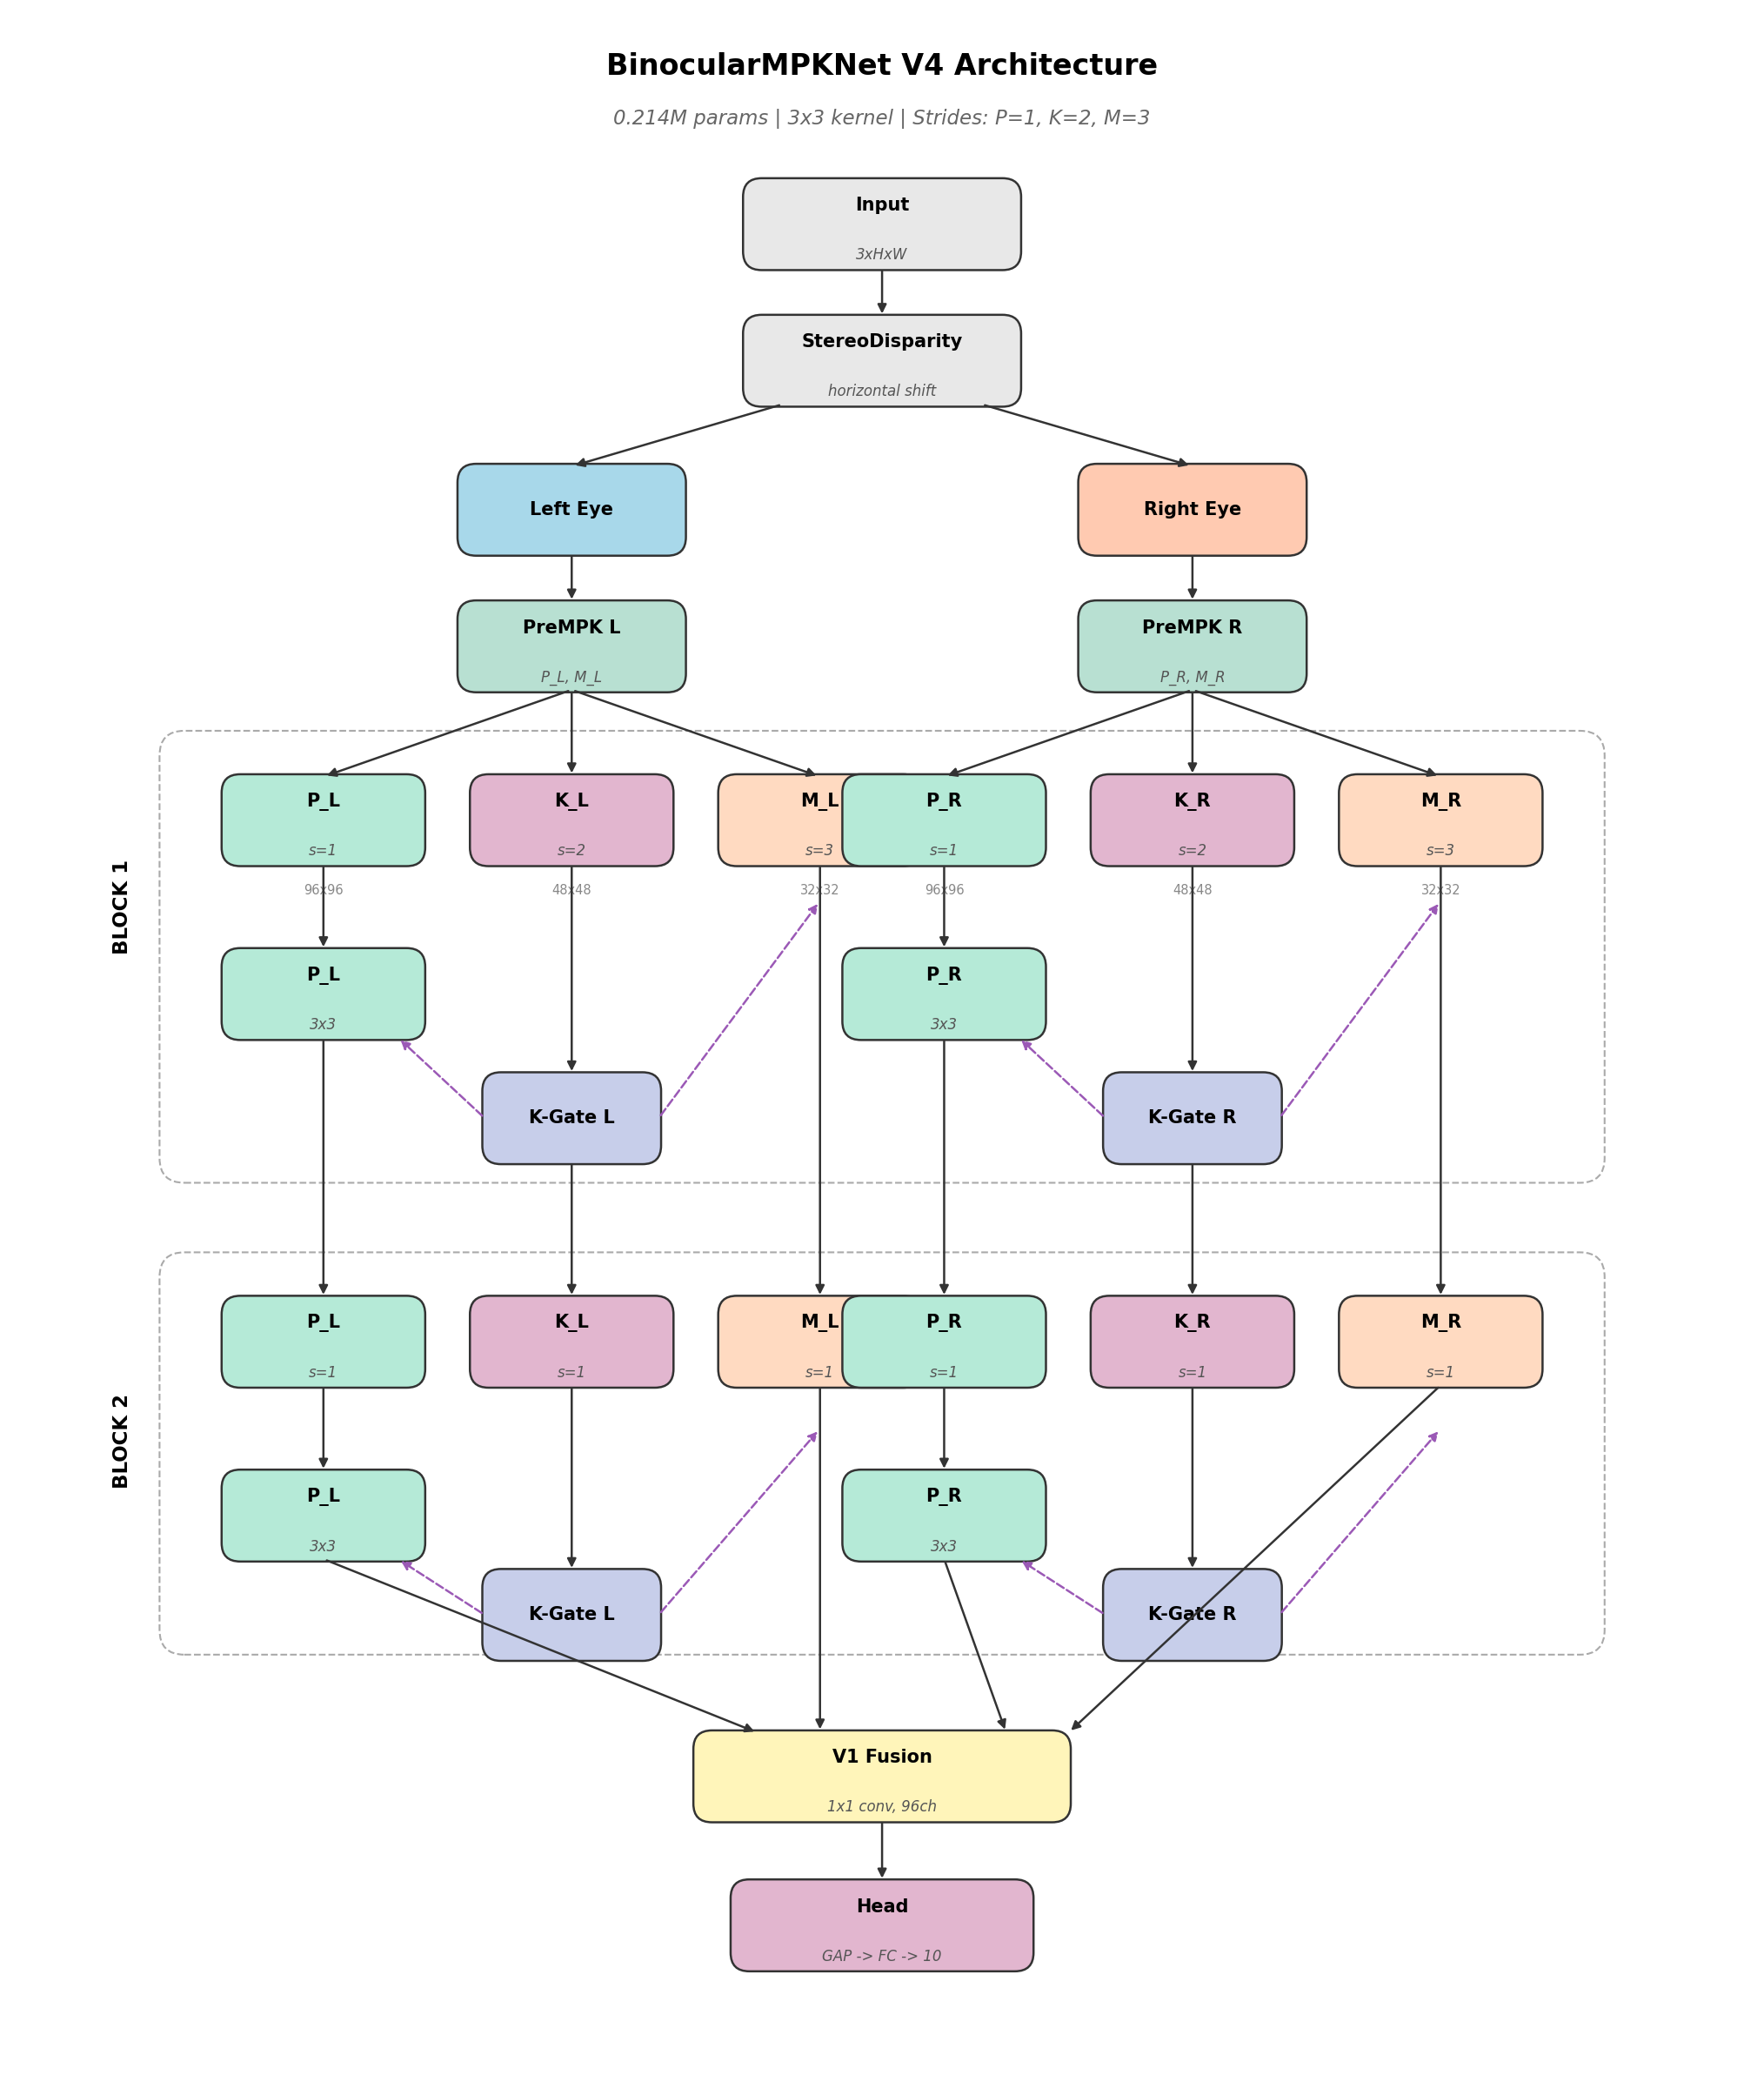
\includegraphics[width=\textwidth]{../figures/binocular_mpknet_v4_architecture.png}
    \caption{Full MPKx architecture showing binocular processing with M, P, and K pathways. Eye segregation persists through LGN blocks, with fusion only at V1.}
    \label{fig:full-arch}
\end{figure}

\begin{figure}[t]
    \centering
    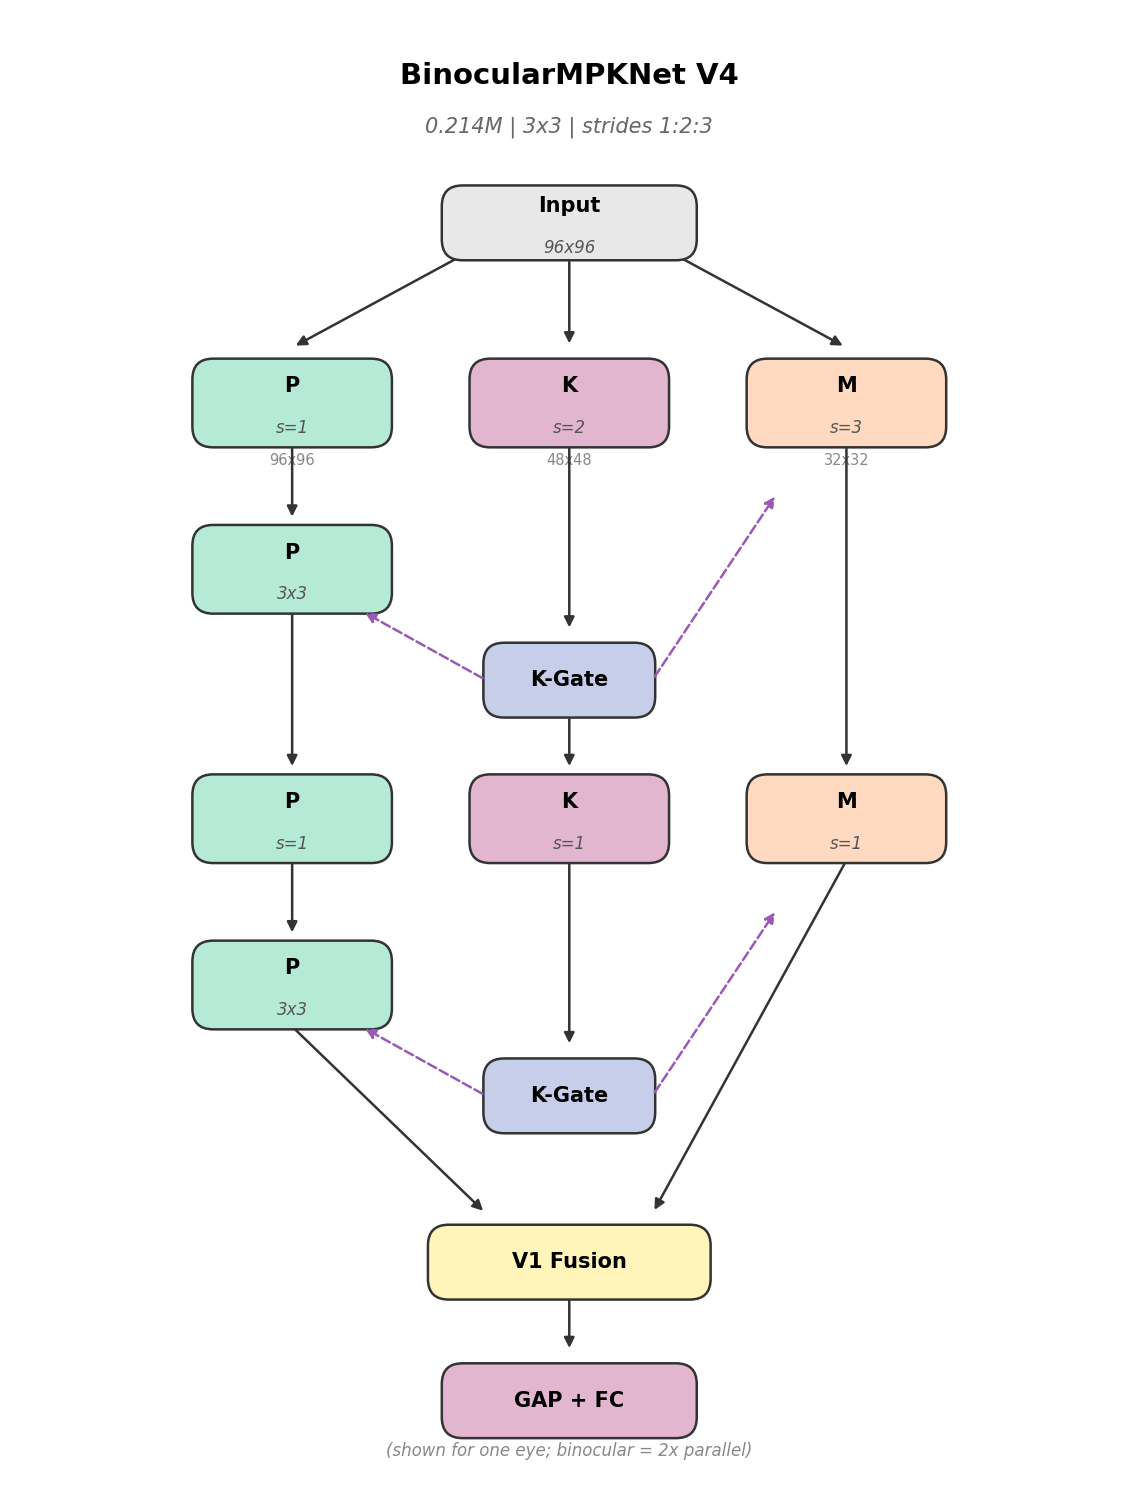
\includegraphics[width=0.8\textwidth]{../figures/binocular_mpknet_v4_simple.png}
    \caption{Simplified view showing the core stride-based pathway differentiation.}
    \label{fig:simple-arch}
\end{figure}

\subsection{Retinal Preprocessing}

Before pathway processing, input images undergo center-surround filtering to simulate retinal ganglion cell responses:
\begin{align}
    P &= I - \text{blur}(I) \quad \text{(high-pass, detail)} \\
    M &= \text{blur}(\text{luminance}) \quad \text{(low-pass, gist)}
\end{align}

This separates the input into P-like (edges, detail) and M-like (global luminance) representations.

\subsection{K-Gating Mechanism}

The K pathway generates channel attention gates:
\begin{align}
    \text{gate}_M &= \sigma(W_M \cdot \text{GAP}(K)) \\
    \text{gate}_P &= \sigma(W_P \cdot \text{GAP}(K)) \\
    M &= M \odot \text{gate}_M \\
    P &= P \odot \text{gate}_P
\end{align}

This implements context-aware gain control, where K acts as a relay that adjusts the relative importance of detail versus global information based on scene content. I suspect K-gating may play a larger role when provided with feedback or feedforward signals from higher visual areas, but that is a hypothesis for future work.

\subsection{Model Summary}

\begin{table}[h]
\centering
\begin{tabular}{ll}
\toprule
\textbf{Metric} & \textbf{Value} \\
\midrule
Parameters & 0.21--0.22M \\
Model size & 0.89MB \\
Embedding size & 96 floats (384 bytes) \\
FLOPs & $\sim$142--280M (task dependent) \\
\bottomrule
\end{tabular}
\caption{Model specifications.}
\label{tab:model-summary}
\end{table}

\section{Experiments}

All experiments were conducted locally on a DGX Spark and/or MacBook M3 Max, using personal hardware. Models were trained from scratch without pretraining, transfer learning, and augmentation. My leading hypothesis is that classification is a trivial task for organisms with a visual system, for instance knowing food that is edible from non-edible. Obviously benchmark datasets are not apples to apples, but the idea is that the sensory features extracted by the MPKx should be rich enough for classification. While also being in my mind being relatively small and metabolic/compute efficient in both training and inference. I have yet to hit SOTA accuracy, but I expect that to change as I continue to learn from research and refining the architecture. I see this as an architectural need, in the sense that vision evolved more complex areas for things like orientation, which may be more useful for classification that expected.

\subsection{Cross-Dataset Results}

\begin{table}[h]
\centering
\begin{tabular}{lccccc}
\toprule
\textbf{Dataset} & \textbf{Params} & \textbf{FLOPs} & \textbf{Test Acc} & \textbf{Acc/Param} & \textbf{Train/Test Gap} \\
\midrule
TinyImageNet & 0.21M & 142M & 40.6\% & 193 & 3.5\% \\
CIFAR-100 & 0.22M & 281M & 58.8\% & 267 & 11\% \\
Kvasir-v2 & 0.21M & 280M & 89.2\% & 425 & 8\% \\
STL-10 & 0.21M & 280M & 71.7\% & 341 & 12\% \\
\bottomrule
\end{tabular}
\caption{All results with no pretraining and no augmentation.}
\label{tab:cross-dataset}
\end{table}

\begin{figure}[t]
    \centering
    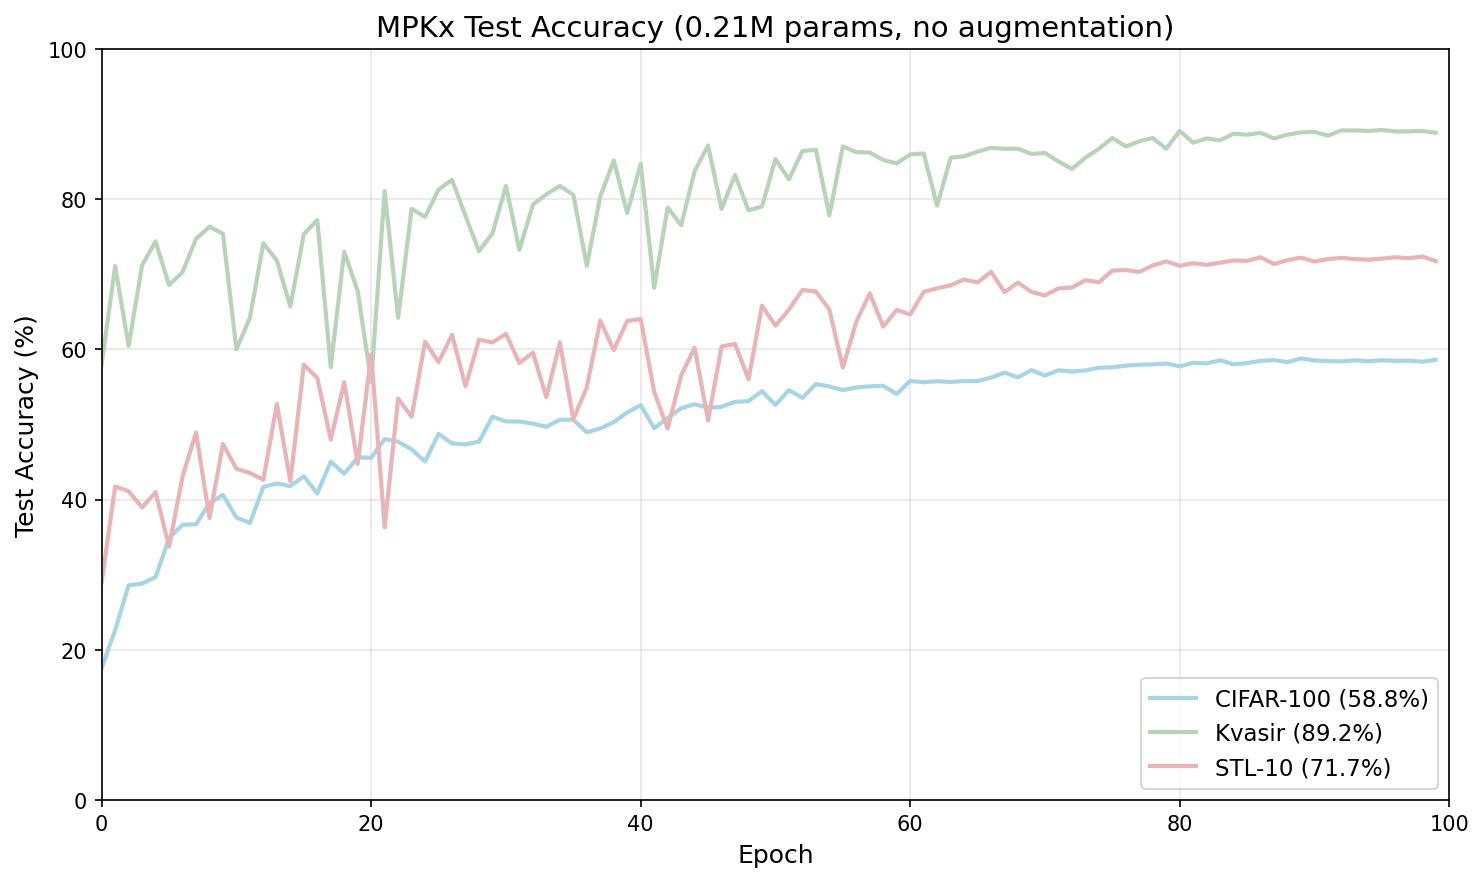
\includegraphics[width=0.9\textwidth]{../figures/v4_training_curves.png}
    \caption{MPKx test accuracy across datasets.}
    \label{fig:training-curves}
\end{figure}

\begin{figure}[t]
    \centering
    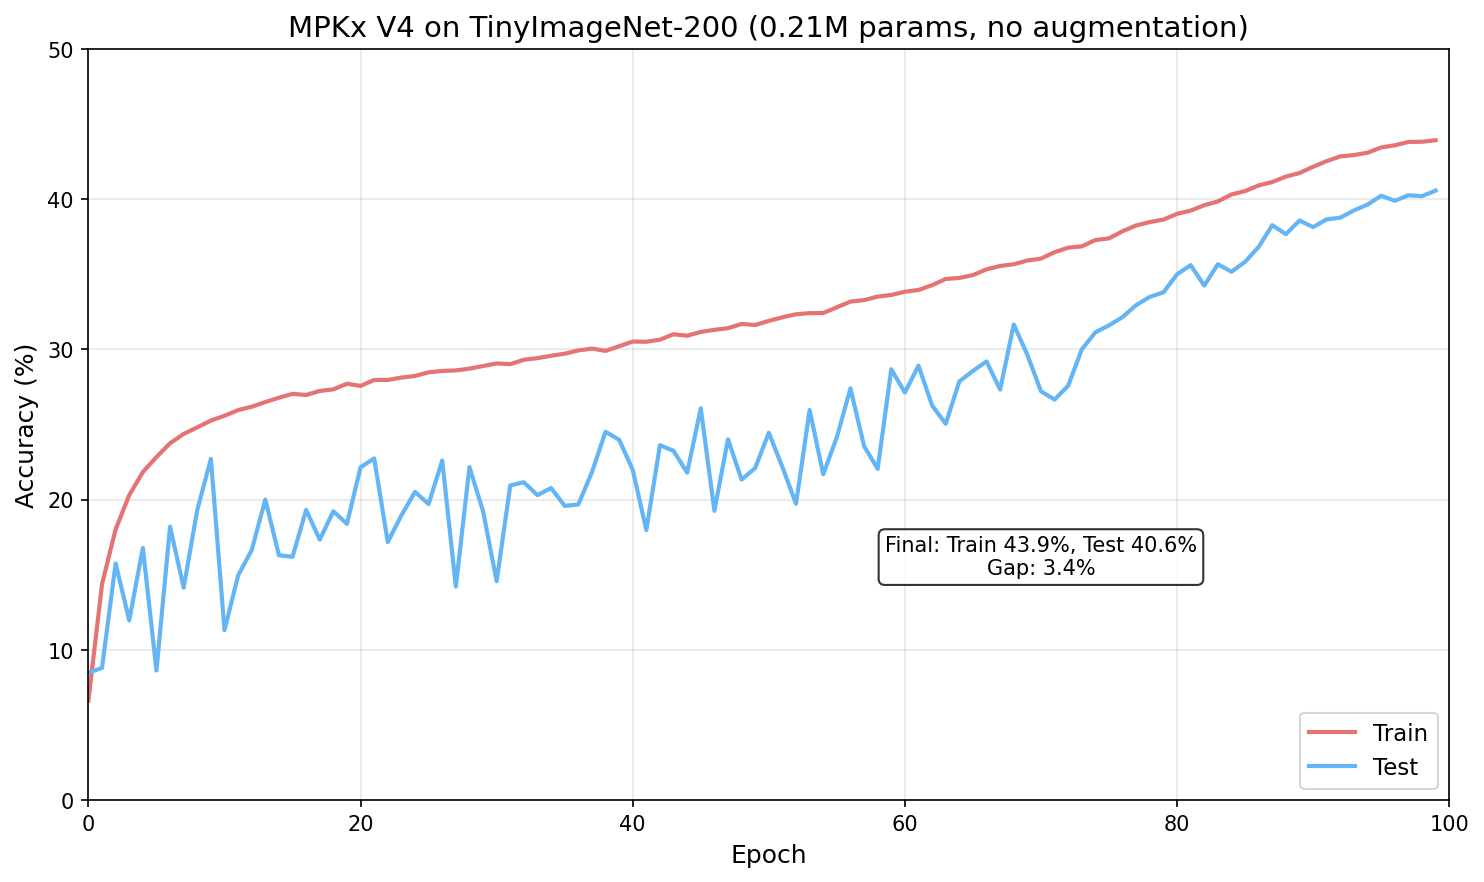
\includegraphics[width=0.9\textwidth]{../figures/tinyimagenet_training_curves.png}
    \caption{TinyImageNet training curves. The train/test gap stays tight ($\sim$3.4\%) throughout training despite no augmentation.}
    \label{fig:tinyimagenet-curves}
\end{figure}

\subsection{TinyImageNet-200 Comparison}

\begin{table}[h]
\centering
\begin{tabular}{lcccc}
\toprule
\textbf{Model} & \textbf{Params} & \textbf{Test Acc} & \textbf{Acc/Param} & \textbf{Notes} \\
\midrule
\textbf{MPKx} & \textbf{0.21M} & \textbf{40.6\%} & \textbf{193} & No augmentation \\
MPKx (with aug) & 0.21M & 24.1\% & 115 & Augmentation hurts \\
ResNet18 & 11M & 41.5\% & 3.8 & 52$\times$ more params \\
MobileNetV2 & 3.4M & 33.1\% & 9.7 & 16$\times$ more params \\
EfficientNet-B0 & -- & 36.9\% & -- & \\
\bottomrule
\end{tabular}
\caption{MPKx matches ResNet18 with 52$\times$ fewer parameters.}
\label{tab:tinyimagenet}
\end{table}

\subsection{Kvasir-v2 (Medical Imaging)}

\begin{table}[h]
\centering
\begin{tabular}{lccc}
\toprule
\textbf{Model} & \textbf{Params} & \textbf{Accuracy} & \textbf{Acc/Param} \\
\midrule
\textbf{MPKx} & \textbf{0.21M} & \textbf{89.2\%} & \textbf{425} \\
ConvMixer & 0.59M & 92.5\% & 157 \\
SqueezeNet & 1.25M & 85.6\% & 68 \\
MobileNetV3-Small & 2.5M & 92.5\% & 37 \\
DenseNet201 & 19.2M & 94.5\% & 5 \\
\bottomrule
\end{tabular}
\caption{89.2\% with no pretraining or augmentation.}
\label{tab:kvasir}
\end{table}

\subsection{Ablation Study}

Need to run proper ablation with new architecture.

\section{Discussion}

\subsection{Why Does Augmentation Hurt?}

The consistent degradation with augmentation (TinyImageNet: -16.5pt; CIFAR-100: -6.8pt) is perhaps the most interesting result. From a neuroscience perspective, this makes sense: the biological visual system has no ``augmentation'' stage. There is no brain region that randomly flips, crops, or color-jitters incoming visual information before processing.

The goal here is for the model to see like a human as much as possible; take in visual information and make sense of it directly. Data augmentation is an engineering trick to compensate for architectural limitations; it teaches invariances that the network cannot learn from structure alone. If the M/P/K architecture already provides those invariances through its parallel processing structure, then augmentation may be adding noise rather than signal.

I do not have a computational explanation for why this happens. But the result is consistent with the design philosophy: build the right structure and let the structure do the work.

\section{Limitations and Future Work}

Several biological features are deliberately omitted:

\begin{itemize}
    \item \textbf{Temporal dynamics}: M cells are more temporally concerned than the P cells who are more spatially concerned. I have not modeled this as I am focusing on static images to get some foundational understanding for the architecture. I however think this is is probably the most important feature to add.
    \item \textbf{Recurrence}: When you get into how areas are connected with each other in the visual system you see it has a variety of feedforward and feedback connections. In particular how the retinal ganglion cells connect to the superior colliculus and then passes back to the LGN via the retinotectal pathway. As well as the network between the LGN and V1, where M, P, and K project to different portions of V1 and then it projects back to the LGN in addition to V2.
\end{itemize}

\subsection{Future Directions}

The current MPKx is just the LGN stage; it can be thought of as early preprocessing before V1. The roadmap is as follows:

\begin{enumerate}
    \item \textbf{LGN} (current): M/P/K parallel pathways. Done.
    \item \textbf{Retinotectal pathway}: Superior colliculus-like saccade generation.
    \item \textbf{V1}: Orientation columns.
    \item \textbf{Thalamo-cortical loops}: Testing whether attention emerges from architecture.
\end{enumerate}

The hypothesis is that attention is not the result of any one set of cells or regions. It emerges from having the right areas connected the right way. Transformers need attention modules because they are missing the architecture that would generate it naturally.

\section{Conclusion}

MPKx demonstrates that biological organizational principles (parallel specialist streams, late fusion) translate to concrete computational advantages. The architecture matches ResNet18 on TinyImageNet with 52$\times$ fewer parameters and exhibits qualitatively different training dynamics, including augmentation insensitivity and tight train/test gaps.

Where computation happens may be as important as what computation happens.

\section*{Acknowledgements}

Thanks to Paul Dassonville (University of Oregon) for telling me about these cells in the first place, and to Jay Pratt (University of Toronto) for ongoing collaboration on koniocellular function.

\bibliographystyle{plainnat}
\begin{thebibliography}{3}

\bibitem[Conley et~al.(1984)]{conley1984}
Conley, M., Fitzpatrick, D., \& Diamond, I.~T. (1984).
\newblock The laminar organization of the lateral geniculate body and the striate cortex in the tree shrew.
\newblock \emph{Journal of Neuroscience}, 4(1), 171--197.

\bibitem[Solomon(2021)]{solomon2021}
Solomon, S.~G. (2021).
\newblock Parallel processing in the visual system.
\newblock \emph{Current Biology}, 31(11), R640--R647.

\bibitem[Yamins et~al.(2014)]{yamins2014}
Yamins, D.~L., Hong, H., Cadieu, C.~F., Solomon, E.~A., Seibert, D., \& DiCarlo, J.~J. (2014).
\newblock Performance-optimized hierarchical models predict neural responses in higher visual cortex.
\newblock \emph{Proceedings of the National Academy of Sciences}, 111(23), 8619--8624.

\end{thebibliography}

\vspace{1em}
\noindent\textit{Patent pending (US 63/950,391)}

\end{document}
